\section{Tree-level, two flavor pion stars}


\subsection{Equation of state}
The free energy density of two-flavor chiral perturbation theory, to leading-order and at $T = 0$, is
%
\begin{equation}
    \Eff = - f^2 \left(\bar m^2 \cos \alpha + \frac{1}{2} \mu_I^2 \sin^2 \alpha\right).
\end{equation}
%
The $\alpha$ parameter is determined by minimizing $\Eff$ for a given value of $\mu_I$,
%
\begin{equation}
    \pdv{\Eff}{\alpha} = f^2 \left(\bar m^2 - \mu_I^2 \cos \alpha\right) \sin(\alpha) = 0.
\end{equation}
%
This gives an explicit formula for $\alpha$ in terms of $\mu_I$.
We are only interested in the phase where $\mu_I \geq \bar m$, where this formula is
%
\begin{align}
    \label{alpha as function of mu lowest order}
    \cos \alpha = \frac{\bar m^2}{\mu_I^2}.
\end{align}
%
We introduce the new dimensionless variable $1 + x^2 = \mu_I^2 / \bar m^2$.
This is reminicent of the dimensionless Fermi momentum $x_f = p_f / m$ in \autoref{section: cold fermi star}. \todo{Tolkning av dette}
By an argument using a right triangle, we can vertify that $\cos a = b$ implies $\sin a = \sqrt{1 - b^2}$.
Substituting the dimensionless variable into the free energy density, we get
%
\begin{equation}
    \Eff = - \frac{u_0}{2}\left(1 + x^2 +\frac{1}{1 + x^2}\right).
\end{equation}
%
We have introduced the characteristic energy density $u_0 = \bar m^2 f^2$.
As we found in \autoref{section: cold fermi star}, pressure is given by negative the free energy density, normalized to $\mu_I = \bar m$, or $x = 0$.
We choose $p_0 = u_0$, so the dimensionless pressure can be written
%
\begin{equation}
    \tilde p = -\frac{1}{u_0}(\Eff - \Eff_{x = 0}) 
    = \frac{1}{2} \frac{x^4}{1 + x^2}.
\end{equation}
%

The charge density corresponding to a chemical potential is given by minus the derivative of the free energy with respect to that chemical potential.
We must, however, not assume any dependence of $\alpha$ on $\mu_I$.
The isospin density therefore is
%
\begin{equation}
    n_I = -\pdv{\Eff}{\mu_I} = f^2 \mu_I \sin^2 \alpha
    = \frac{u_0}{\mu_I} \frac{2x^2 + x^4}{1 + x^2}.
    ,
\end{equation}
%
With this, the dimensionless energy density
%
\begin{equation}
    \tilde u = -\tilde p + \frac{1}{u_0} n_I \mu_I
    = \frac{1}{2} \frac{4x^2 + x^4}{1 + x^4}
\end{equation}
%
This is illustrated in \autoref{fig: equation of state pions tree level}

\begin{figure}[h]
    \centering
    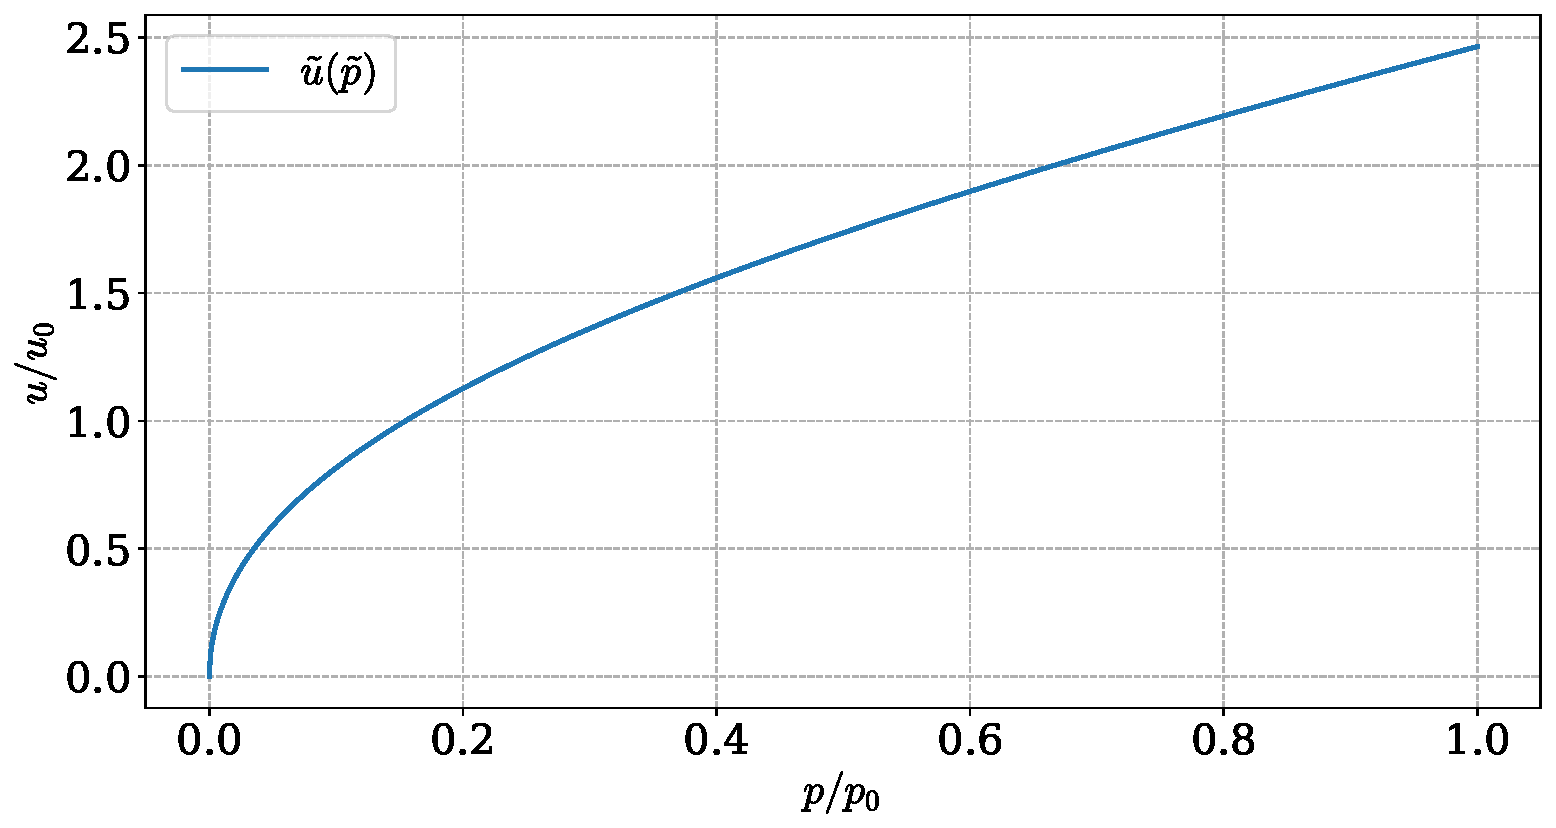
\includegraphics[width=0.6\textwidth]{../scripts/figurer/pion_tree_eos.pdf}
    \caption{
        This plot shows the tree-level equation of state of two-flavor chiral perturbation theory. The $x$-axis shows the pressure normalized to $p_0$, while the $y$-axis shows the energy density normalized to $u_0$.
        }
        \label{fig: quation of state pions tree level}
\end{figure}


\subsection{Units}

The characteristic mass and length, as discussed in \autoref{section: TOV equation}, are found by setting $k_1 = k_2 = k_3 = 1$.
These are the dimensionless constants of the TOV equation, \autoref{dimensionless constants TOV}.
At tree-level, the bare constants $f$ and $\bar m$ are related to physical constants by $f = f_\pi$ and $m = m_\pi$, the pion decay constant and the pion mass.
Using the values for $f_\pi$ and $m_\pi$ as given in \autoref{section: units} and reinstating $c$ and $\hbar$, these quantities are give in SI-units by
%
\begin{align}
    u_0 & =m_\pi^2 f_\pi^2 \frac{c}{\hbar^3}
    = 3.216\cdot 10^{33} \, \text{J}\,\text{m}^{-3}, \\
    m_0 & = \frac{c^4}{\sqrt{\frac{4 \pi}{ 3} u_0 G}} = 64.21\, M_\odot, \\
    r_0 & = \frac{G}{c^2} m_0 = 94.79 \, \text{km}.
\end{align}
%
We therefore expect both the radius and mass of the pion star to be around one order of magnitude larger than the star made up of cold neutrons.


\subsection{Results}

The code used for obtaining numerical results is discussed in \autoref{appendix: code}.

\autoref{fig: pressure and mass for tree-level pion star} show the pressure and mass as a function of radius for a range of central pressures.
The quantities are normalized to the stellar radius, stellar mass, and central pressure, respectively.
The black dashed line corresponds to the configuration with the maximum mass.
We see that both the pressure and mass distribution are very similar for stars with a mass less than the maximum.

\autoref{fig: mass radius relation tree-level pion star} shows the mass-radius relationship for the pion star using the tree-level free energy density of two-flavor chiral perturbation theory.
As in the case of the neutron star, it has a maximum mass, in this case of $M_\text{max} 10.47\, M_\odot$.
What distinguishes this from the case of the neutron star, however, is the fact that in the limit of low central pressure, the distribution apparently approaches a maximum radius of $R = 85.95 \, \text{km}$.
\todo{Hvorofor? Fordi eos er så lite stiv?}



\begin{figure}[h]
    \centering
    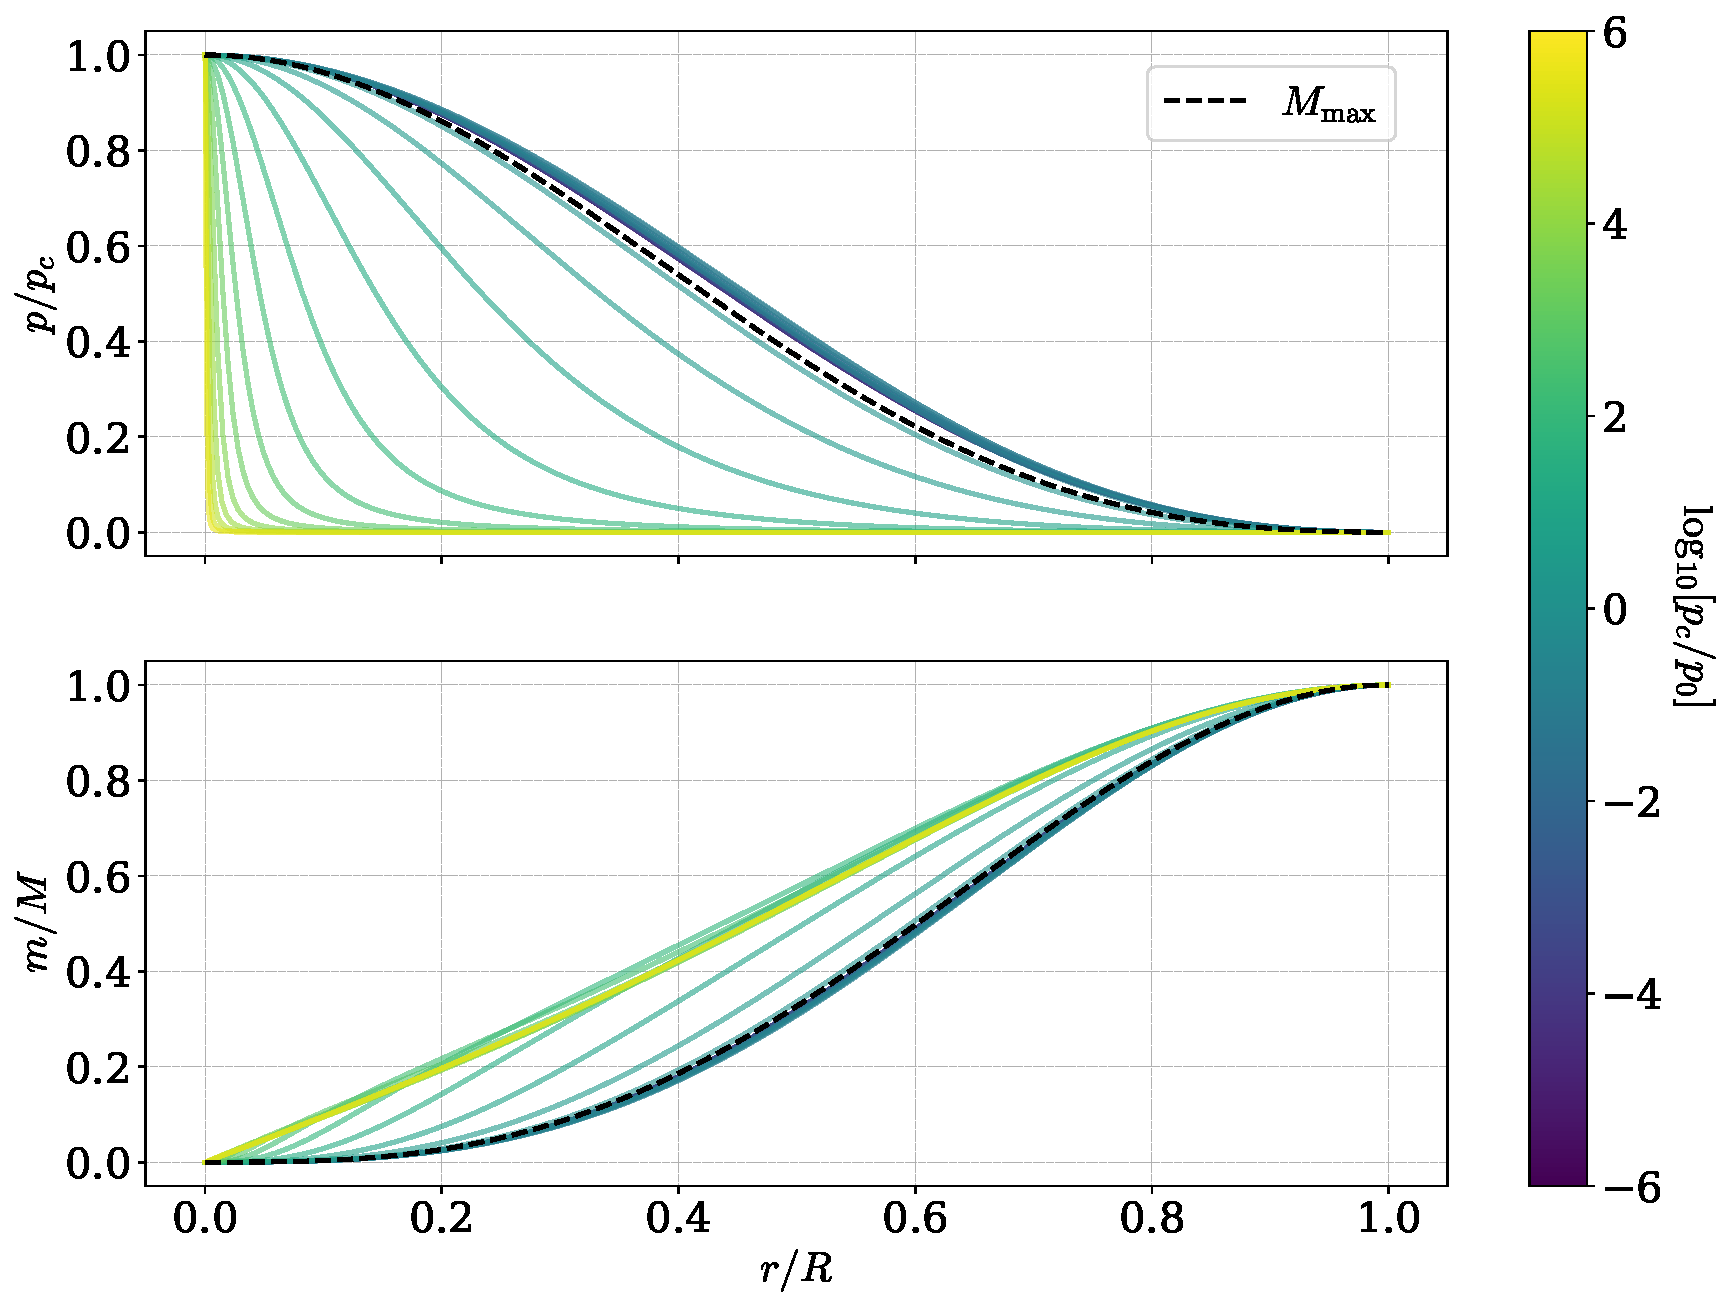
\includegraphics[width=0.8\textwidth]{../scripts/figurer/pressure_mass_pion_star.pdf}
    \caption{
        Top: The pressure normalized to the central pressure, as a function of radius, normalized to the stellar radius.
    Bottom: The mass, normalized to stellar mass, within a radius $r$, normalized to the stellar radius.
    Both plots show a range of stars with different central pressures, indicated by the color range.
    The black dotted line corresponds to the star with the largest mass.}
    \label{fig: pressure and mass for tree-level pion star}
\end{figure}


\begin{figure}[h]
    \centering
    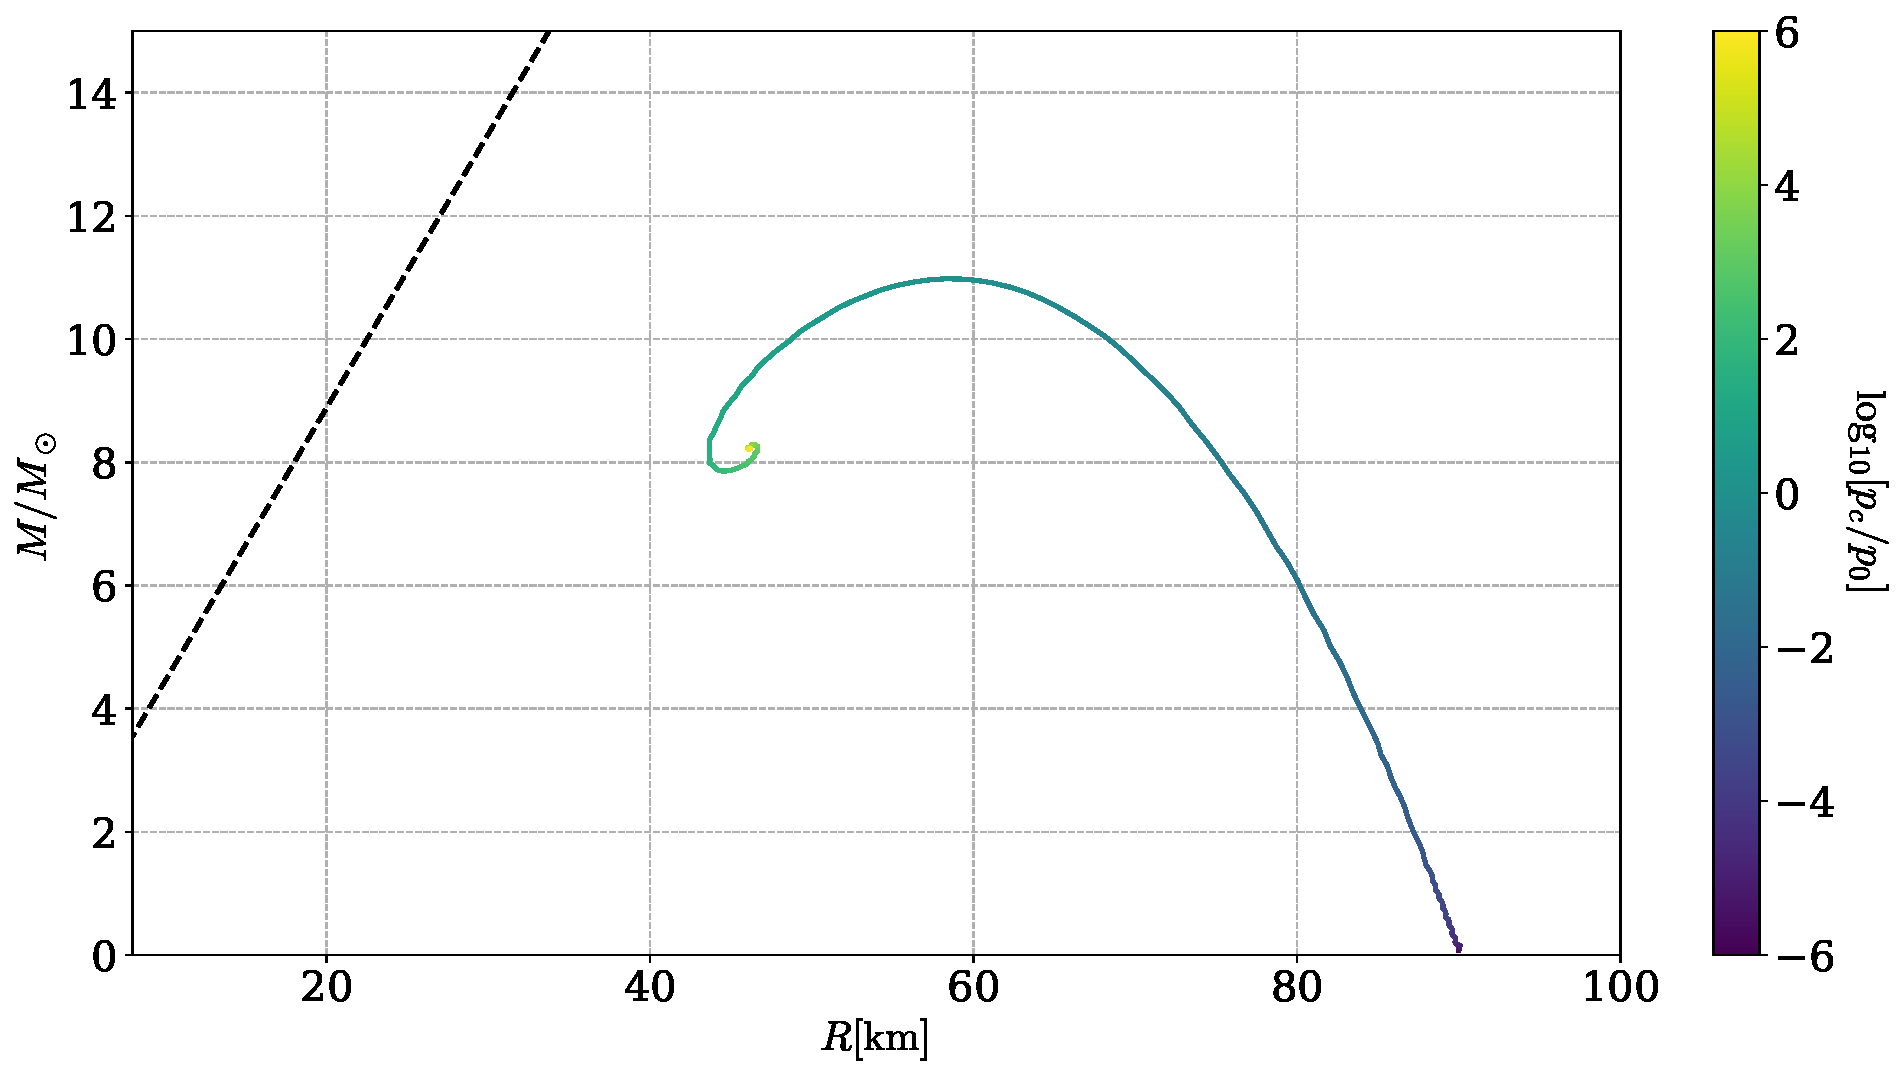
\includegraphics[width=0.95\textwidth]{../scripts/figurer/mass_radius_pion_star_tree.pdf}
    \caption{
        The plot shows the relationship between the mass and radius of a pion star. Mass is given in units of solar masses, while the radius is measured in kilometers.
        This line is parameterized by the central pressure $p_c$ of the star, as indicated by the color gradient.
        The dashed black line indicates the theoretical maximum mass for a given radius, and the configuration above it will collapse to a black hole.
        }
        \label{fig: mass radius relation tree-level pion star}
\end{figure}

